%! TEX root = ../main.tex
% ============================================================
% IMMUTABLE — generated automatically, do not edit this block
%   script          : plotter.py
%   plot_type       : parallel_ratio
%   chapter         : 04
%   panel           : None
%   wind            : None
%   amplitude       : None
%   frequency       : None
%   probes          : None
%   draft           : True
%
% DATASETS:
%   PROCESSED-20260326-ProbePos4_31_FPV_2-tett6roof-under9Mooring-height100-lowrange
%   PROCESSED-20260327-ProbePos4_31_FPV_2-tett6roof-under9Mooring30-height100-lowrange
%
% SUBFIGURES AVAILABLE:
%   FIGURES/ch04_parallel_ratio_scatter.pdf
% ============================================================
\begin{figure}[htbp]
  \centering
  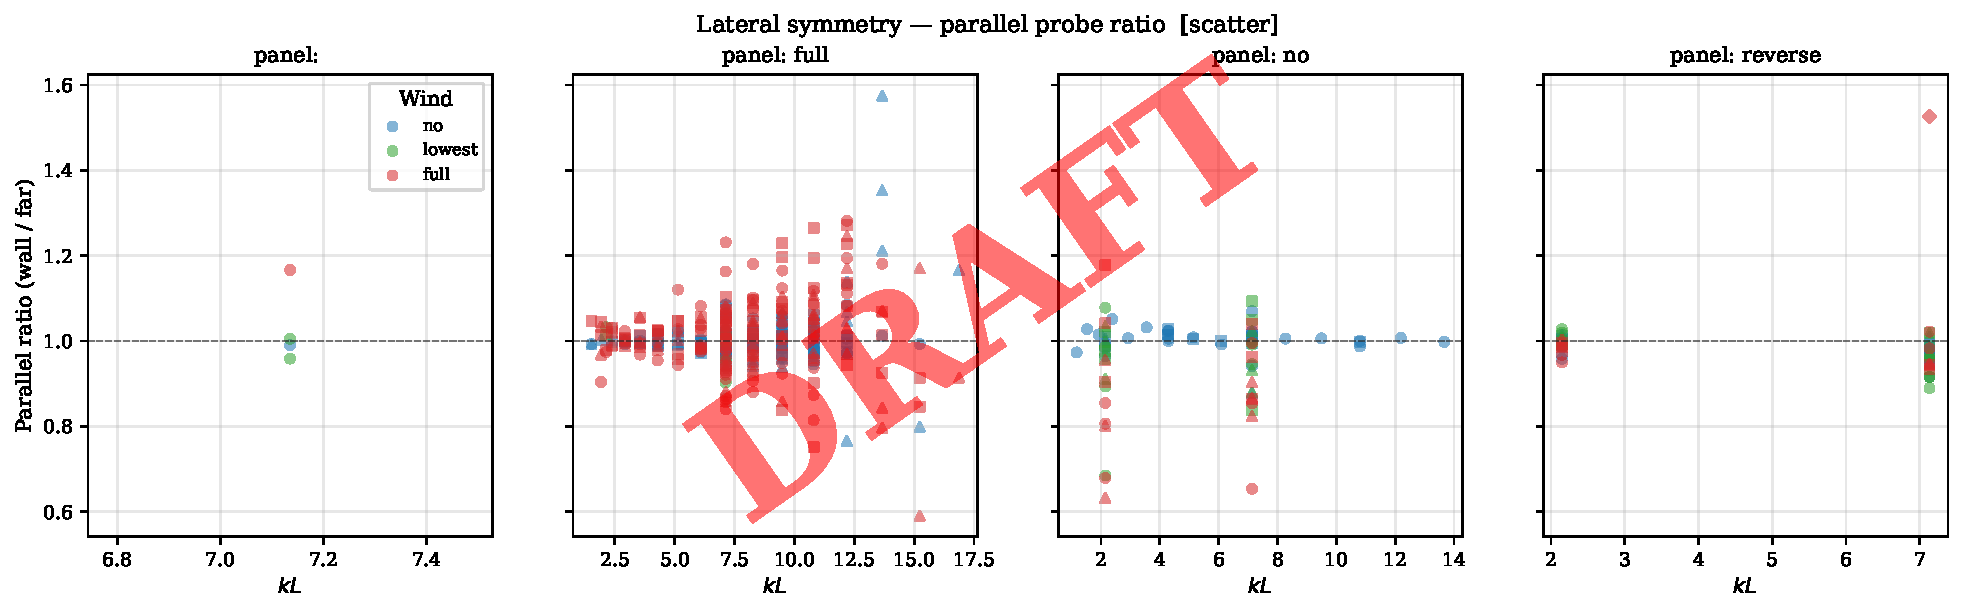
\includegraphics[width=0.9\linewidth]{FIGURES/ch04_parallel_ratio_scatter.pdf}
  \caption[Same data as the parallel-ratio figure, plotted as individual run points (no grouping)]{
    Same data as the parallel-ratio figure, plotted as individual run points (no grouping). Each dot = one run. Colour = wind condition; marker shape = wave amplitude. Use to identify outlier runs.
  }
  \label{fig:ch04_parallel_ratio_scatter}
\end{figure}
